% Scalar instruction entry source: tools/generate_scalar_instruction_catalog.py.
\subsection{\texttt{CMP.EQ}}
\label{sec:scalar-cmp_eq}
\index{CMP.EQ@\texttt{CMP.EQ}}
\begin{sloppypar}\noindent\textbf{Purpose.} Compares SrcL and the modified SrcR for equality and writes 1 or 0 to RegDst.\end{sloppypar}\smallskip
\noindent\textbf{Syntax.}\par
\begin{lstlisting}[style=ptoscalarcode]
cmp.eq SrcL, SrcR<{.sw, .uw}>, ->RegDst
\end{lstlisting}
\noindent\textbf{Encoding.}\par
\noindent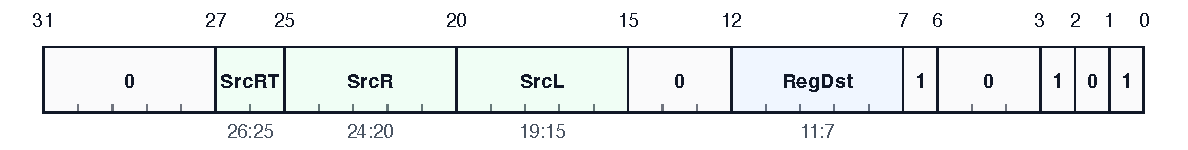
\includegraphics[width=\textwidth]{figs/encoding/scalar_instruction_entries/enc_cmp_eq.pdf}\par\smallskip
\begin{description}[leftmargin=0.18\linewidth,style=nextline]
\item[Format] \texttt{L32} \texttt{32-bit} scalar word.
\item[Pattern] \texttt{00000............000.....1000101}.
\end{description}
\noindent\textbf{Classification.}\par
\begin{description}[leftmargin=0.18\linewidth,style=nextline]
\item[Category] Branch, Compare, and PC Control.
\item[Family] Compare Instruction.
\item[Execution class] \texttt{BRU}; uop\_kind=BRU, bru\_kind=CMP.
\end{description}
\noindent\textbf{Operand fields.}\par
\begin{description}[leftmargin=0.18\linewidth,style=nextline]
\item[\texttt{RegDst}] Bits \texttt{11:7 (5b)}. 5-bit scalar destination register that receives the boolean compare result, encoded as 1 for true and 0 for false; X0 discards the write.
\item[\texttt{SrcL}] Bits \texttt{19:15 (5b)}. 5-bit scalar source register used as the left operand of the comparison.
\item[\texttt{SrcR}] Bits \texttt{24:20 (5b)}. 5-bit scalar source register used as the right operand of the comparison before any SrcRType modifier is applied.
\item[\texttt{SrcRType}] Bits \texttt{26:25 (2b)}. 2-bit modifier for SrcR. It selects the encoded source form shown in the syntax, such as signed-word, unsigned-word, negated, or unmodified register input.
\end{description}
\noindent\textbf{Operation.}\par
\begin{lstlisting}[style=ptoscalarcode]
result = (Read(SrcL) == Read(SrcR)) ? 1 : 0
Write(RegDst, result)
\end{lstlisting}
\Needspace{0.08\textheight}
